\section{Tab-Navigation}
Andere mit React Native gebauten Apps, wie Facebook oder Instagram, verwenden eine sogenannte
"Bottom-Tabs"{}-Navigation, also eine Tab-Basierte Navigation auf der Unterseite des Bildschirms, um
ihre Hauptfunktionen dem Benutzer zu präsentieren.

Um die App simpel zu halten ist dies auch unsere präferierte Navigations-Methode, um die einzelnen
Bereiche der Anwendung miteinander zu verbinden.

\begin{lstlisting}
import MapScreen from '../screens/MapScreen';
import ProfileScreen from '../screens/ProfileScreen';
import SkateparksStack from './SkateparksStack';
import Colors from '../styles/Colors';

const Tab = createBottomTabNavigator();

const BottomTabsNavigator = () => {
  const tabBarIcons = (route, focused, color) => {
    ...
  };

  return (
    <Tab.Navigator
      backBehavior="initialRoute"
      initialRouteName="Skateparks"
      screenOptions={({ route }) => ({
        tabBarIcon: ({ focused, color }) => tabBarIcons(route, focused, color),
        tabBarActiveTintColor: Colors.primary,
        tabBarInactiveTintColor: Colors.gray2,
        tabBarActiveBackgroundColor: Colors.primarySoft,
        tabBarShowLabel: false,
        headerShown: false,
      })}
    >
      <Tab.Screen name="Skateparks" component={SkateparksStack} />
      <Tab.Screen name="Map" component={MapScreen} />
      <Tab.Screen name="Profile" component={ProfileScreen} />
    </Tab.Navigator>
  );
};

export default BottomTabsNavigator;
\end{lstlisting}

In Zeile 14 wird aus dem Objekt Tab zuerst der Navigator und danach, als Kinder, die einzelnen
Screens eingefügt. Als Screens können hierbei weitere andere Navigatoren verwendet werden, um eine
Verschachtelung zu erzeugen.

\subsection{MapScreen}
Die Umsetzung der Kartenfunktion, um alle Skateparks anzuzeigen, war das zweit-komplizierteste
Feature in der App. Die Bibliothek \textbf{react-native-maps} ist hierbei die Basis dieser Funktion.

\begin{code}[htp]
\begin{lstlisting}[firstnumber=1,language=JavaScript, style=JSX]
const MapScreen = ({ navigation }) => {
  const {
    data: skateparks,
    isLoading,
    error,
    refreshData,
  } = useFetch('https://skate-buddy.josholaus.com/api/skateparks');
  const mapRef = useRef(null);

  return (
    <View style={styles.container}>
      {isLoading && <LoadingCircle />}
      {error && <Error error={error} refresh={refreshData} />}
      {skateparks && (
        <>
          <Map
            mapRef={mapRef}
            skateparks={skateparks}
            navigation={navigation}
          />
          <CircleButton
            onPress={() => {
              mapRef.current.animateCamera({
                center: {
                  latitude: 47.27,
                  longitude: 11.4,
                },
                altitude: 1000,
                pitch: 0,
                heading: 0,
                zoom: 12,
              });
            }}
          />
        </>
      )}
    </View>
  );
};
export default MapScreen;
\end{lstlisting}
\caption{React Component - Der Karten-Tab}
\end{code}

Zuerst werden mit dem Hook \textbf{useFetch} alle Skateparks von der API abgefragt, solange die Variable
\textbf{skateparks} \textbf{null} ist, wird nur ein Ladesymbol angezeigt. Anschließend wird die Map erzeugt, wie auch
ein Knopf, mit dem man die Position der Karte auf Innsbruck zentrieren kann.

\begin{figure}[H]
  \begin{center}
    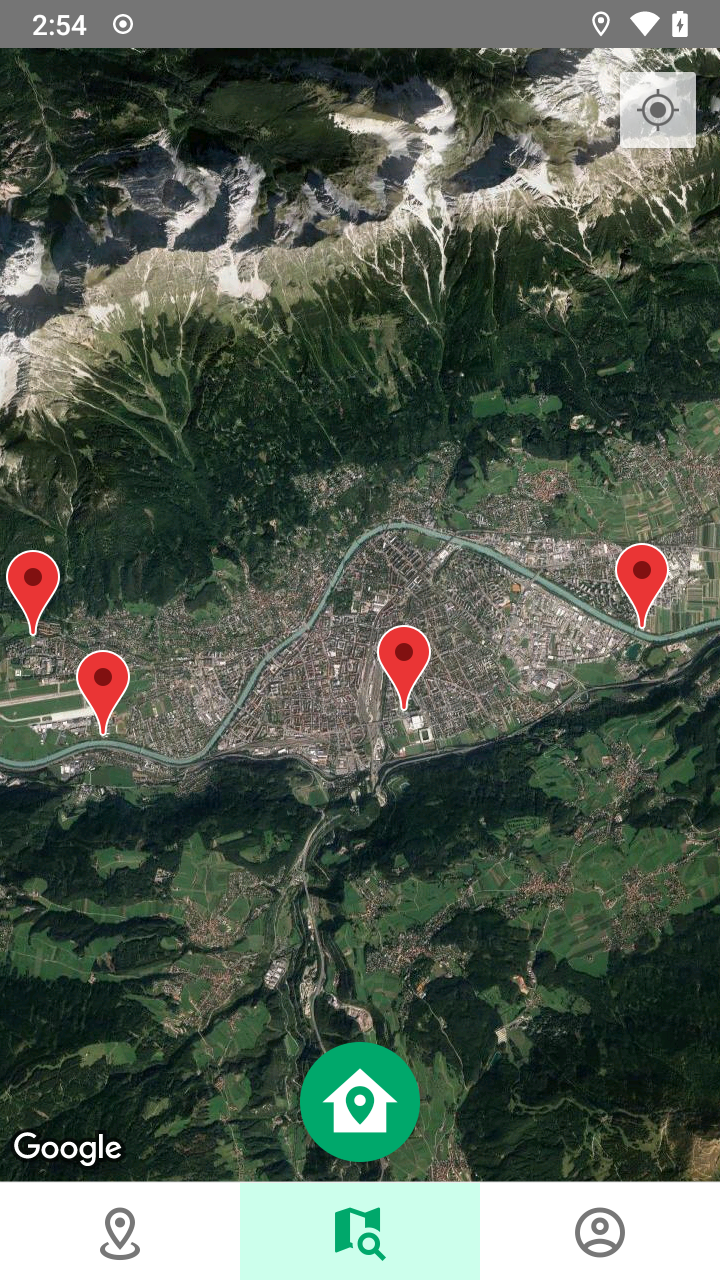
\includegraphics[width=0.6\textwidth]{Mobile/Map/MapScreen.png}
    \caption{Alle Skateparks werden an der korrekten Position angezeigt}
  \end{center}
\end{figure}

\newpage
\subsubsection{Map}

\begin{code}[htp]
\begin{lstlisting}[firstnumber=1,language=JavaScript, style=JSX]
const Map = ({ skateparks, mapRef, navigation }) => {
  return (
    <MapView
      // props
      showsUserLocation
      provider={PROVIDER_GOOGLE}
      style={mapStyles.map}
      ref={mapRef}
      initialCamera={camera}
      showsPointsOfInterest={false}
      showsCompass={false}
      showsIndoors={false}
      minZoomLevel={8}
      rotateEnabled={false}
      pitchEnabled={false}
      mapType="satellite"
    >
      <SkateparkMarkers
        skateparks={skateparks}
        mapRef={mapRef}
        navigation={navigation}
      />
    </MapView>
  );
};
export default Map;
\end{lstlisting}
\caption{React Component - Die MapView-Komponente aus react-native-maps}
\end{code}

In der Komponente \textbf{Map} wird einfach eine \textbf{MapView} aufgerufen, welche die Google Maps Ansicht
beinhaltet. Die Parks werden anschließend wieder an die nächste Komponente weitergegeben, wo sie in
die Map-Marker umgewandelt werden. Drückt man auf einen Marker, so wird der Park zentriert und ein
Textfeld wird angezeigt. Wird dies angeklickt, so wird man zu den Details vom jeweiligen Park
weitergeleitet.

\begin{figure}[H]
  \begin{center}
    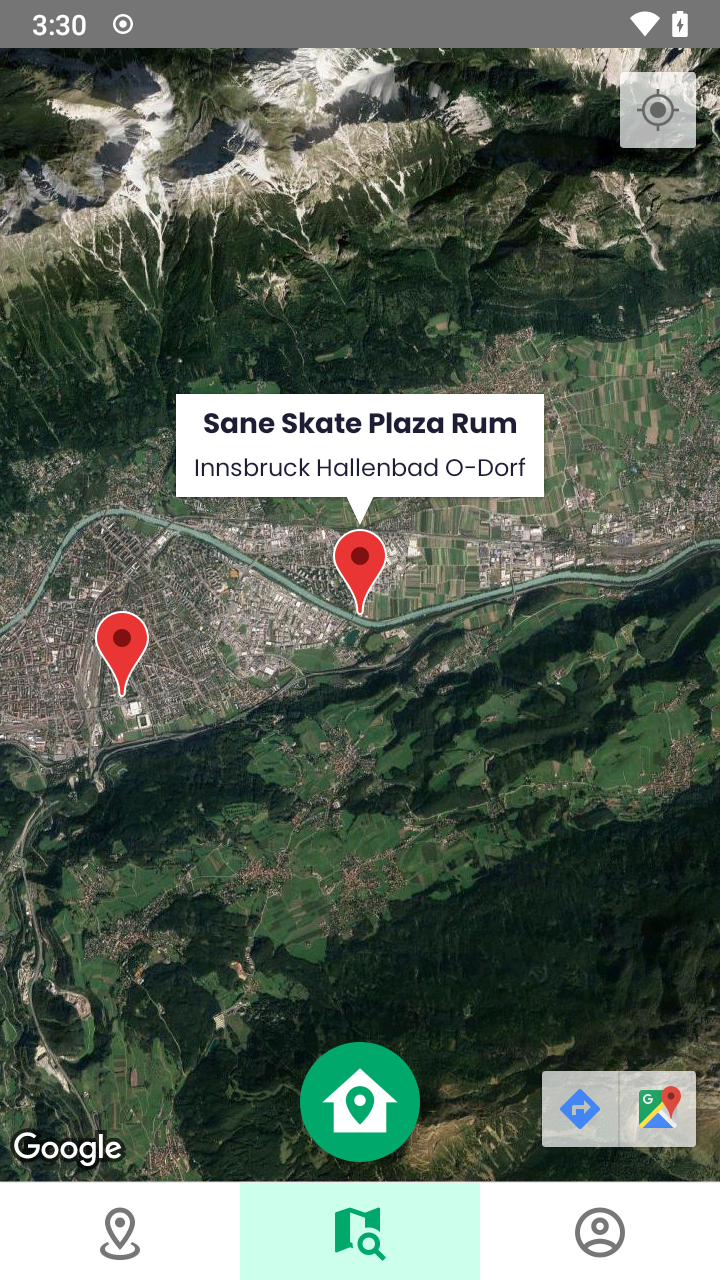
\includegraphics[width=0.6\textwidth]{Mobile/Map/MapMarkerFocused.png}
    \caption{Ein ausgewählter Marker}
  \end{center}
\end{figure}

\subsection{ProfileScreen}
In der Profilansicht werden lediglich einige Informationen zum User, ein Standard-Profilbild und
ein Knopf, zum Ausloggen, angezeigt.

\begin{figure}[H]
  \begin{center}
    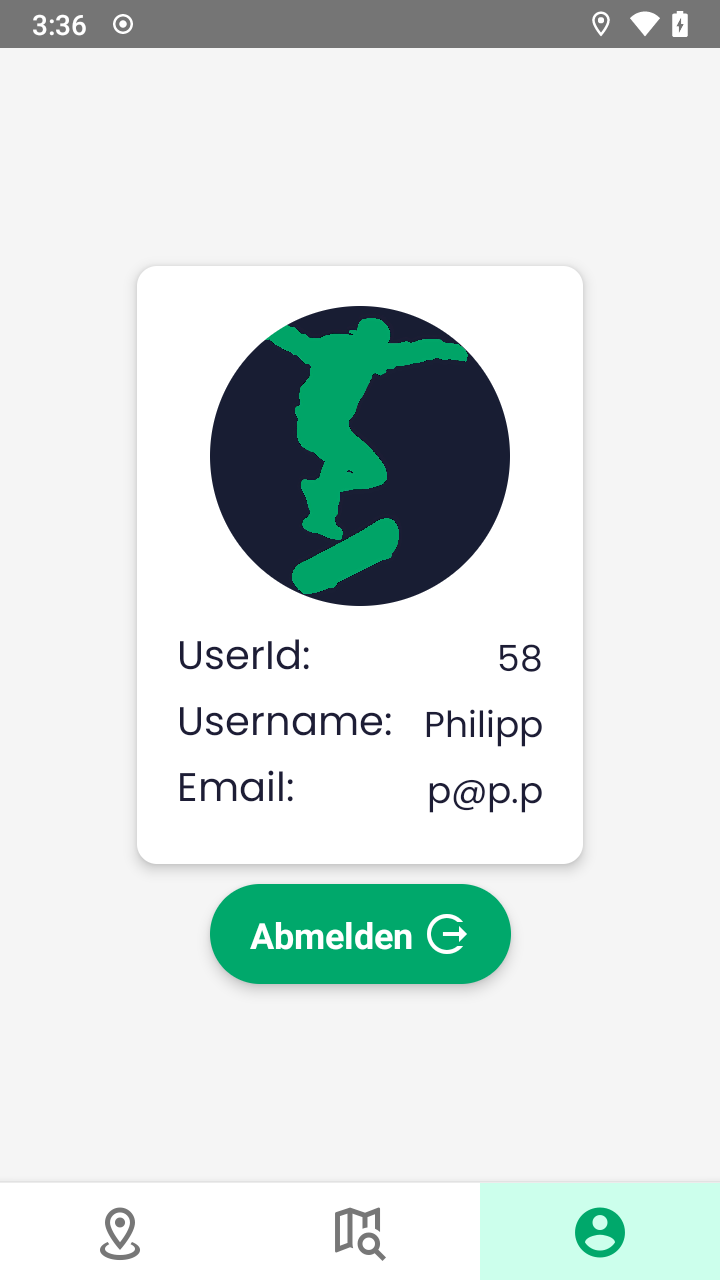
\includegraphics[width=0.6\textwidth]{Mobile/ProfileScreen.png}
    \caption{Die Profil-Ansicht}
  \end{center}
\end{figure}
